\documentclass[11pt]{article}
\usepackage{fullpage,amsthm,amssymb,tikz,amsmath,verbatim,mathtools}

\begin{document}

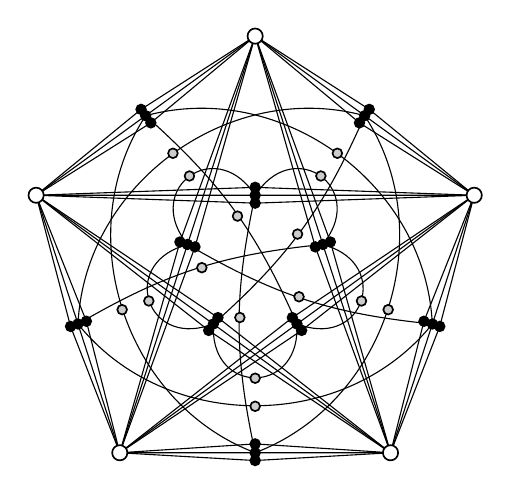
\begin{tikzpicture}[scale=.65]
\tikzstyle{uStyle}=[shape = circle, minimum size = 5.5pt, inner sep = 0pt,
outer sep = 0pt, draw, fill=white, semithick]
\tikzstyle{lStyle}=[shape = circle, minimum size = 4.5pt, inner sep = 0pt,
outer sep = 0pt, draw, fill=none, draw=none]
\tikzstyle{usStyle}=[shape = circle, minimum size = 3.5pt, inner sep = 0pt,
outer sep = 0pt, draw, fill=black, semithick]
\tikzstyle{usGStyle}=[shape = circle, minimum size = 3.5pt, inner sep = 0pt,
outer sep = 0pt, draw, fill=gray!40!white, semithick]
\tikzset{every node/.style=uStyle}
\def\rad{4.5cm}

\foreach \i in {1,2,3,4,5}
\draw (\i*72+18:\rad) node[] (x\i) {};
\draw (0,0) node[draw=none] (origin) {};

% ``outside edges''
\foreach \i/\j in {1/2, 2/3, 3/4, 4/5, 5/1}
{
\draw (x\i) -- (barycentric cs:x\i=5,x\j=5,origin=-.4) node[usStyle] {} -- (x\j);
\draw (x\i) -- (barycentric cs:x\i=5,x\j=5,origin=0) node[usStyle] (y\i) {} -- (x\j);
\draw (x\i) -- (barycentric cs:x\i=5,x\j=5,origin=.5) node[usStyle] {} -- (x\j);
}

% ``diagonals''
\foreach \i/\j in {1/3, 2/4, 3/5, 4/1, 5/2}
{
\draw (x\i) -- (barycentric cs:x\i=3,x\j=3,origin=-.6) node[usStyle] {} -- (x\j);
\draw (x\i) -- (barycentric cs:x\i=3,x\j=3,origin=0) node[usStyle] (z\i) {} -- (x\j);
\draw (x\i) -- (barycentric cs:x\i=3,x\j=3,origin=.75) node[usStyle] {} -- (x\j);
}

\foreach \i/\j in {1/3, 2/4, 3/5, 4/1, 5/2}
{
\draw (y\j) edge[bend left=50] (y\i);
\draw (barycentric cs:y\i=3,y\j=3,origin=-3.53) node[usGStyle] {};
\draw (y\i) edge[bend left=12] (z\j);
}

\foreach \i/\j/\k in {1/3/5, 2/4/1, 3/5/2, 4/1/3, 5/2/4}
\draw (barycentric cs:y\i=3,z\j=3.35,y\k=.6) node[usGStyle] {};

\foreach \i/\j in {1/2, 2/3, 3/4, 4/5, 5/1}
\draw (z\j) edge[bend left=90, looseness=2] (z\i);

\foreach \i in {1,...,5}
\draw (barycentric cs:y\i=3,origin=2.0) node[usGStyle] {};

\end{tikzpicture}

\end{document}